\subsection{Opening the \caesarj -perspective}
First of all you need to open the \caesarj -perspective. It includes some new features like the \caesar -editor, the new outline view or the \caesarj -hierarchy view.\\
You can open this perspective by selecting: \markedtext{Window} $\rightarrow$ \markedtext{Open Perspective} $\rightarrow$ \markedtext{other} $\rightarrow$ \markedtext{CaesarJ perspective}.\\
If this is the first time you used the plugin, you will see the following dialog popup shown in figure \ref{fig:view_properties}.

\begin{figure}[htbp]
	\centering
		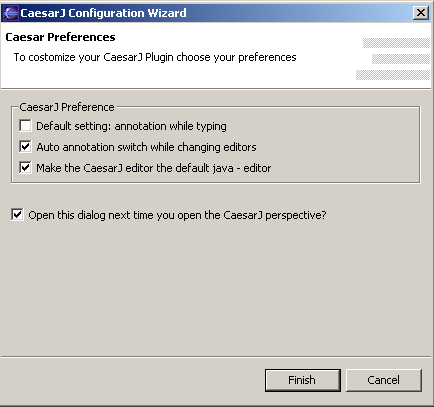
\includegraphics[width=0.5\textwidth]{images/view_properties.png}
	\caption{The \caesarj ~Preferences}	
	\label{fig:view_properties}
\end{figure}

This dialog configures some Eclipse settings that will make your life much easier when
working with \caesarj -projects. Leave everything selected and click
\markedtext{Finish}.

\subsection{Creating a new \caesarj project \label{creating_project}}
From the File menu select \markedtext{New} $\rightarrow$ \markedtext{Project}. Pick \markedtext{Caesar Project} in the list and select \markedtext{Next} as shown in figure \ref{fig:project_wizard}.

\begin{figure}[htbp]
	\centering
		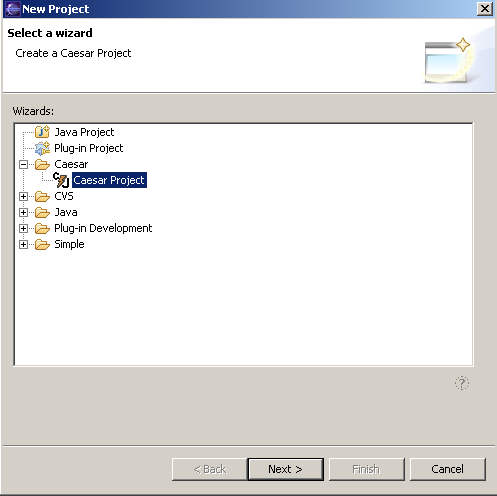
\includegraphics[width=0.60\textwidth]{images/project_wizard.png}
	\caption{Coosing the New Project Wizard}
	\label{fig:project_wizard}
\end{figure}

If it doesn't appear in the list, this is probably the first time you use the plugin. Select \markedtext{Other} and then \markedtext{Caesar} and \markedtext{Caesar Project}.\\
The wizard is opened. Here specify a name for your project as shown in figure \ref{fig:project_wizard2}.

\begin{figure}[htbp]
	\centering
		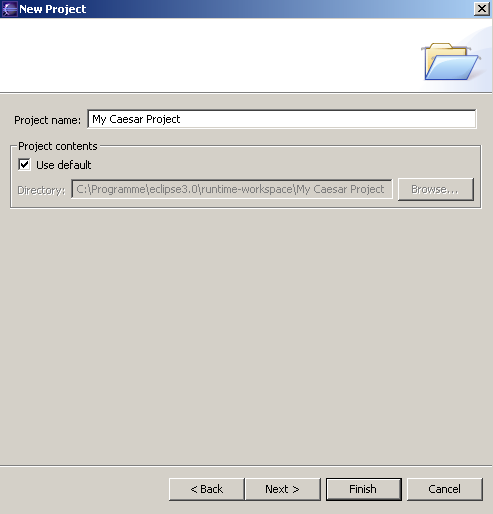
\includegraphics[width=0.60\textwidth]{images/project_wizard2.png}
	\caption{The New Project Wizard}
	\label{fig:project_wizard2}
\end{figure}

This wizard has identical behavior to the new Java project wizard (except of course that
it creates a project with the Caesar nature).\\
When you click \markedtext{Finish}, your project will be created.